\section{Results}
	\subsection{Descriptive Analysis}

	\subsection{ARIMA model}
	\paragraph{Time series decomposition}The time series of total dengue cases in Thailand was additively decomposed in the components trend, seasonal and random, as shown in Figure \ref{fig:decomp_ts_dengue}. The time series shows a seasonal pattern with a frequency of 12 months. The trend shows fluctuation over the time period with two periods of comparatively high dengue cases. 
	
	\begin{figure}[htbp] 
		\centering
		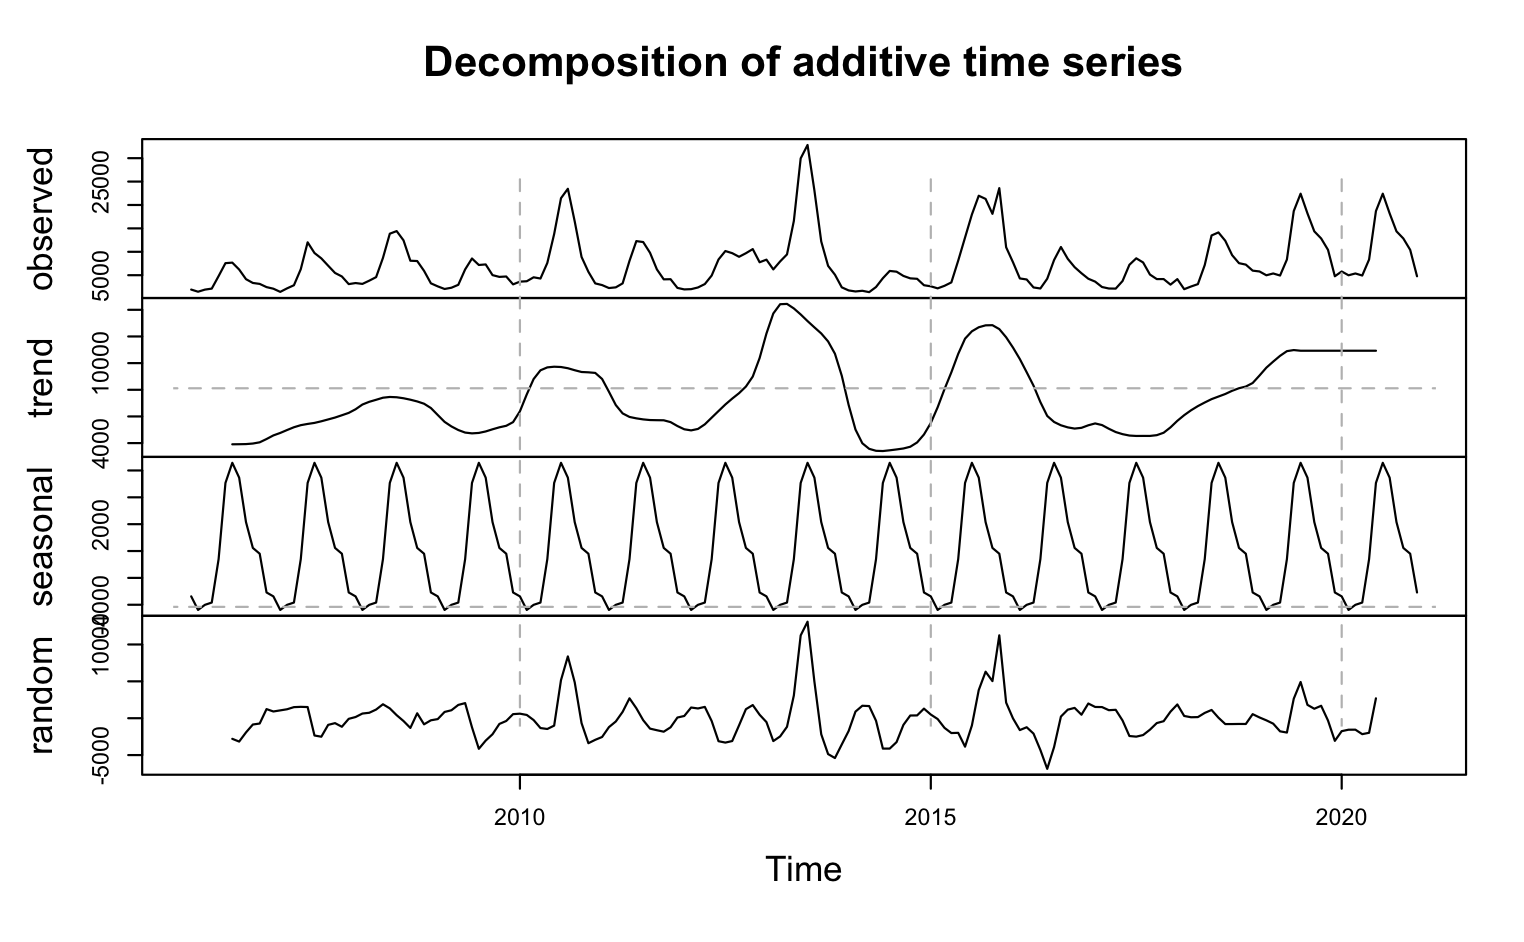
\includegraphics[width=0.7\textwidth]{fig/Decomposition_of_add_ts.png}
		\caption{ Decomposition of the additive time series of the total dengue cases in Thailand}
		\label{fig:decomp_ts_dengue}
	\end{figure}
	
	The decomposition of the time series of the dengue cases was compared to the decomposition of the time series of temperatures. Both time series have an annual seasonal pattern. The trends show in general similar patterns with differences in the amplitudes and slight shifts on the time axis, as shown in Figure \ref{fig:Trend_temp_cases}.
	\begin{figure}[hbpt] 
		\centering
		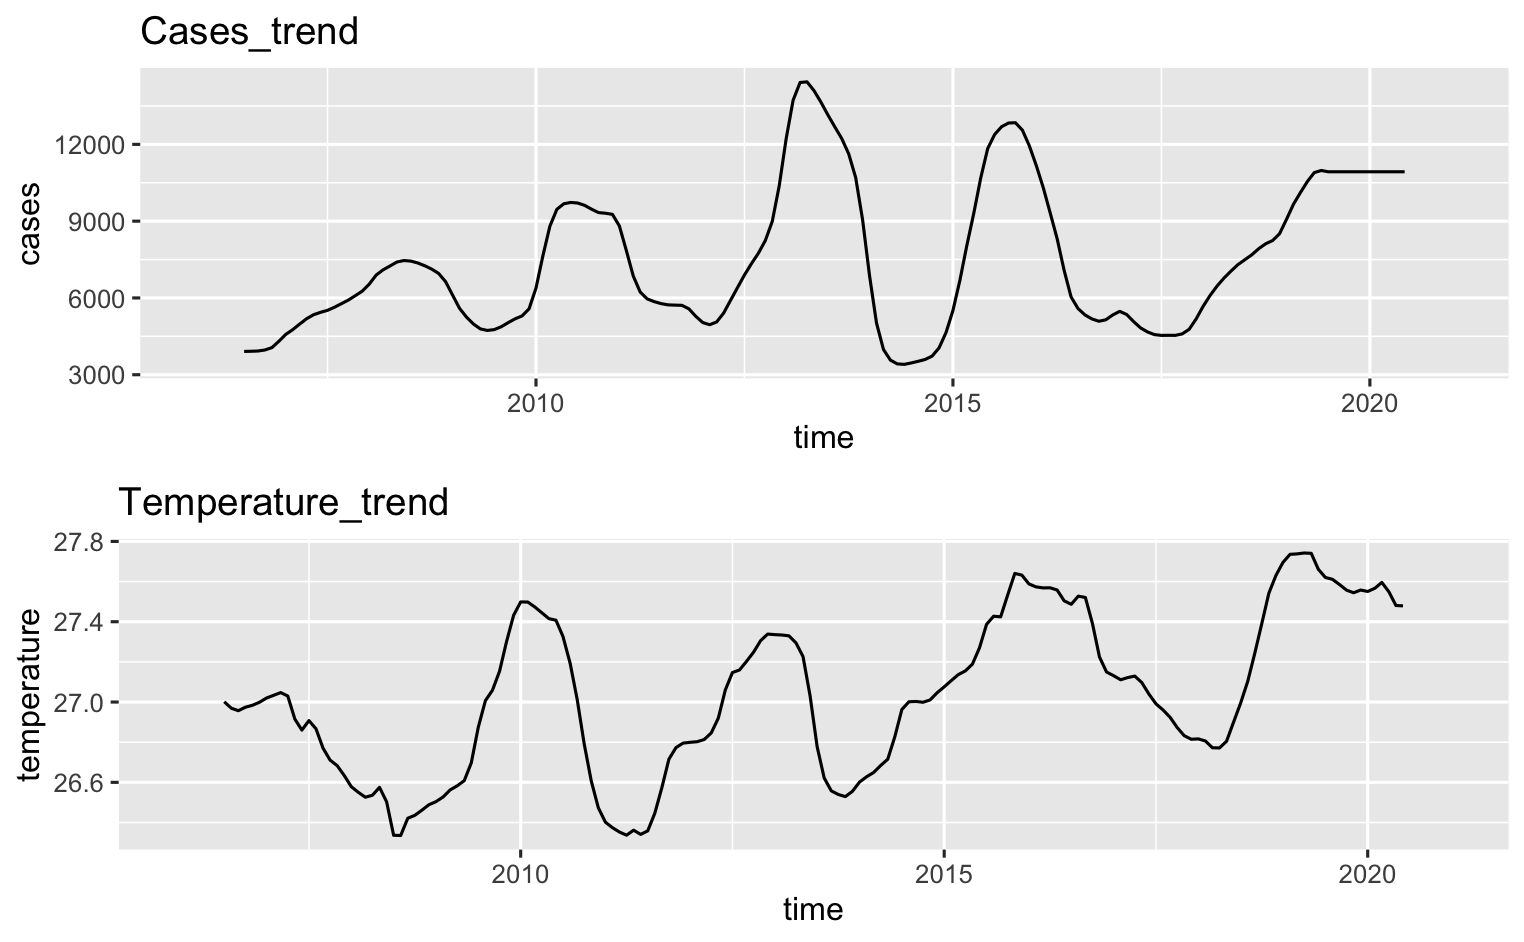
\includegraphics[width=0.7\textwidth]{fig/Trend_temp_cases.png}
		\caption{Trend of the total dengue cases in Thailand compared to the trend of the average temperature in Thailand for the years 2006 till 2020.}
		\label{fig:Trend_temp_cases}
	\end{figure}
	
	\paragraph{ARIMA forecast}
	
	